%%%% APÊNDICE -- TELAS DAS APLICAÇÕES IRIS
%%
%% Reúne as capturas de tela do IRIS web e do IRIS Mobile organizadas por
%% módulo funcional. As capturas foram deslocadas do Capítulo de
%% Desenvolvimento para o apêndice de modo a preservar a fluidez do texto e
%% evitar interrupções gráficas extensas no corpo das subseções.

\chapter{Telas das aplicações IRIS \emph{web} e IRIS \textit{Mobile}}\label{cap:apendiceTelas}

Este apêndice reúne as capturas das principais telas das duas aplicações cliente desenvolvidas para o experimento --- o IRIS \emph{web}, generalista, e o IRIS \textit{Mobile}, especializado na captura de biossinais ---, discutidas respectivamente nas Seções~\ref{sec:desenvolvimentoIRIS} e~\ref{sec:desenvolvimentoIRISMobile}. As capturas reproduzem o estado das aplicações contra um NPI alimentado com os dados do experimento descrito no Capítulo~\ref{cap:desenvolvimento} e foram deslocadas para apêndice de modo a preservar a continuidade da leitura textual sem prejuízo do registro visual das interfaces resultantes.

A organização do apêndice acompanha a estrutura modular discutida no capítulo principal. A Seção~\ref{sec:apendiceTelasIRIS} apresenta as telas do IRIS \emph{web} agrupadas por módulo funcional --- gestão de acessos, gestão de rótulos, gestão de voluntários, gestão de pesquisas e federação ---, enquanto a Seção~\ref{sec:apendiceTelasIRISMobile} percorre as cinco telas mais representativas do IRIS \textit{Mobile} na ordem em que tipicamente são acionadas durante uma coleta. Em ambas as seções, optou-se por preservar o agrupamento das figuras em sub-figuras (\textit{subfloats}) sempre que o módulo correspondente reuni\-a múltiplas variantes de uma mesma tela, evidenciando a coerência do sistema de \textit{design} adotado.

% ----------------------------------------------------------------------
\section{Telas do IRIS \emph{web}}\label{sec:apendiceTelasIRIS}
% ----------------------------------------------------------------------

Esta seção apresenta uma tela representativa de cada módulo funcional do IRIS \emph{web} (Subseção~\ref{subsec:IRISModulos}). A exposição inicia-se pela tela de gestão de acessos, que serve de referência para os padrões visuais reaproveitados nos módulos seguintes, e progride na ordem em que os elementos são tipicamente acionados pelo pesquisador --- da configuração inicial à operação corrente da federação.

A Figura~\ref{fig:irisTelaAcessos} materializa o padrão de listagem paginada adotado em todo o IRIS \emph{web}: barra de busca acima da tabela, ação primária de criação à direita do cabeçalho e ações secundárias por linha (visualização e edição, sinalizadas pelos ícones de olho e lápis). A própria tela --- intitulada \emph{Usuários e Pesquisadores} --- ilustra ainda o uso de abas para segregar conjuntos relacionados de dados em uma mesma visão: a aba \emph{Usuários} (a) lista as contas de acesso da instituição com as colunas \emph{Login}, \emph{Tipo}, \emph{Pesquisador} e \emph{Último acesso}, enquanto a aba \emph{Pesquisadores} (b) expõe o cadastro institucional propriamente dito (Nome, Email, Instituição, Tipo e ORCID), separando a identidade de autenticação da identidade científica do indivíduo. A tela de gestão de rótulos (Figura~\ref{fig:irisTelaRotulos}) reaproveita o mesmo padrão de listagem e o mesmo recurso de abas para organizar o vocabulário clínico em quatro visões complementares --- uma para cada entidade SNOMED CT manipulada pelo NPI . Em todas as telas a coluna \emph{Código SNOMED} é exibida ao lado do termo legível, evidenciando ao usuário que cada rótulo está vinculado a uma referência canônica externa, e não a uma cadeia de caracteres livre.

\begin{figure}[htb]
\caption{Tela de gestão de acessos do IRIS \emph{web}, organizada em duas abas que unificam o cadastro institucional: (a) aba \emph{Usuários}, com as contas de acesso ao sistema; (b) aba \emph{Pesquisadores}, com o cadastro científico dos pesquisadores vinculados à instituição.}
\label{fig:irisTelaAcessos}
\centering
\subfloat[Usuários cadastrados]{
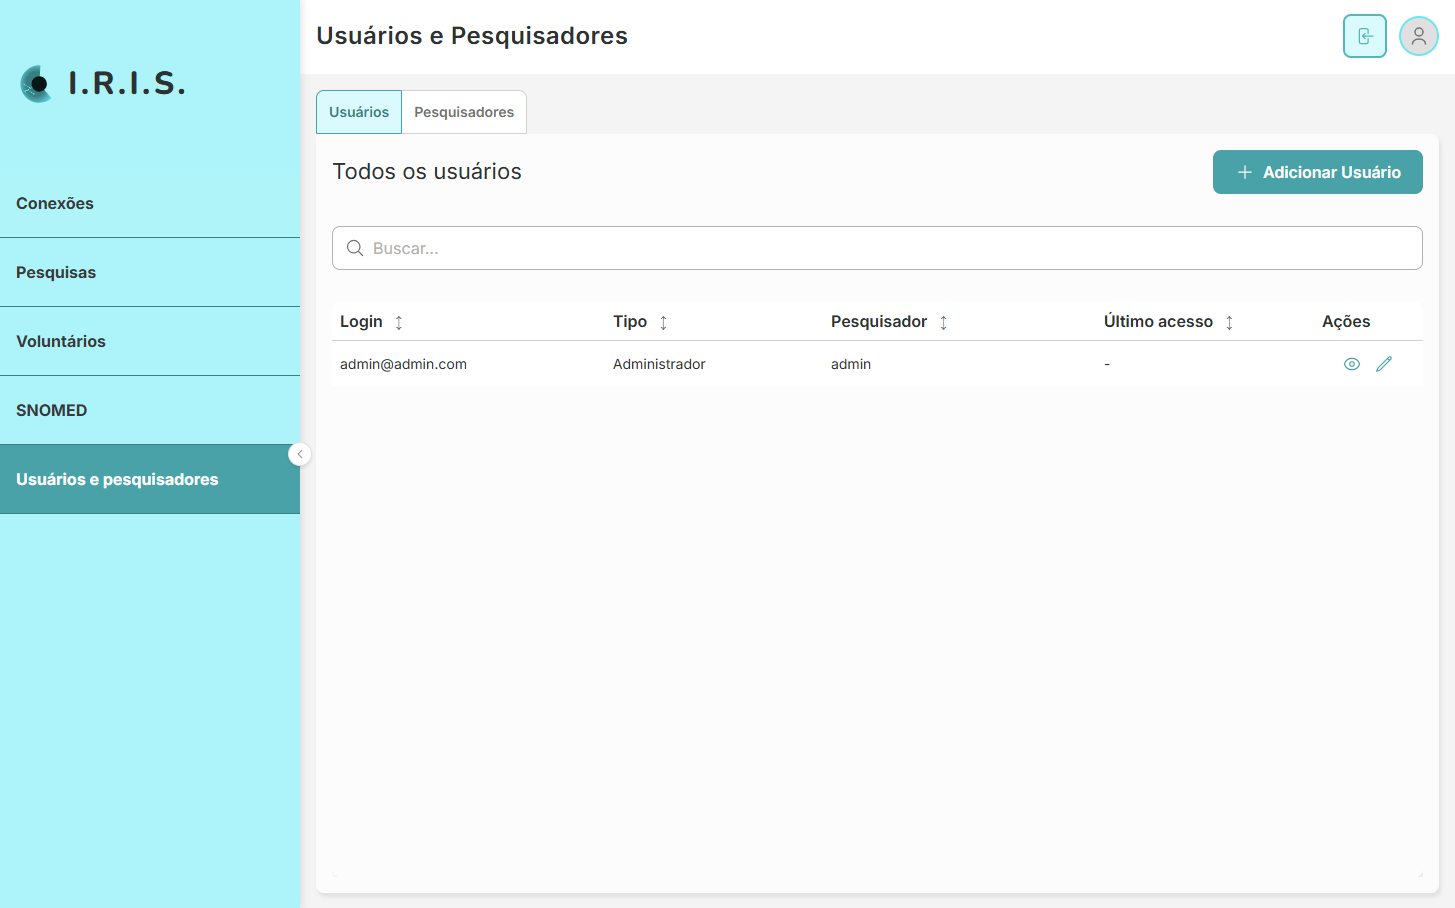
\includegraphics[scale=0.30]{figuras/Desenvolvimento/IRIS/screens/gestao-acessos-usuarios.png}
}\hspace{0.15cm}
\subfloat[Pesquisadores cadastrados]{
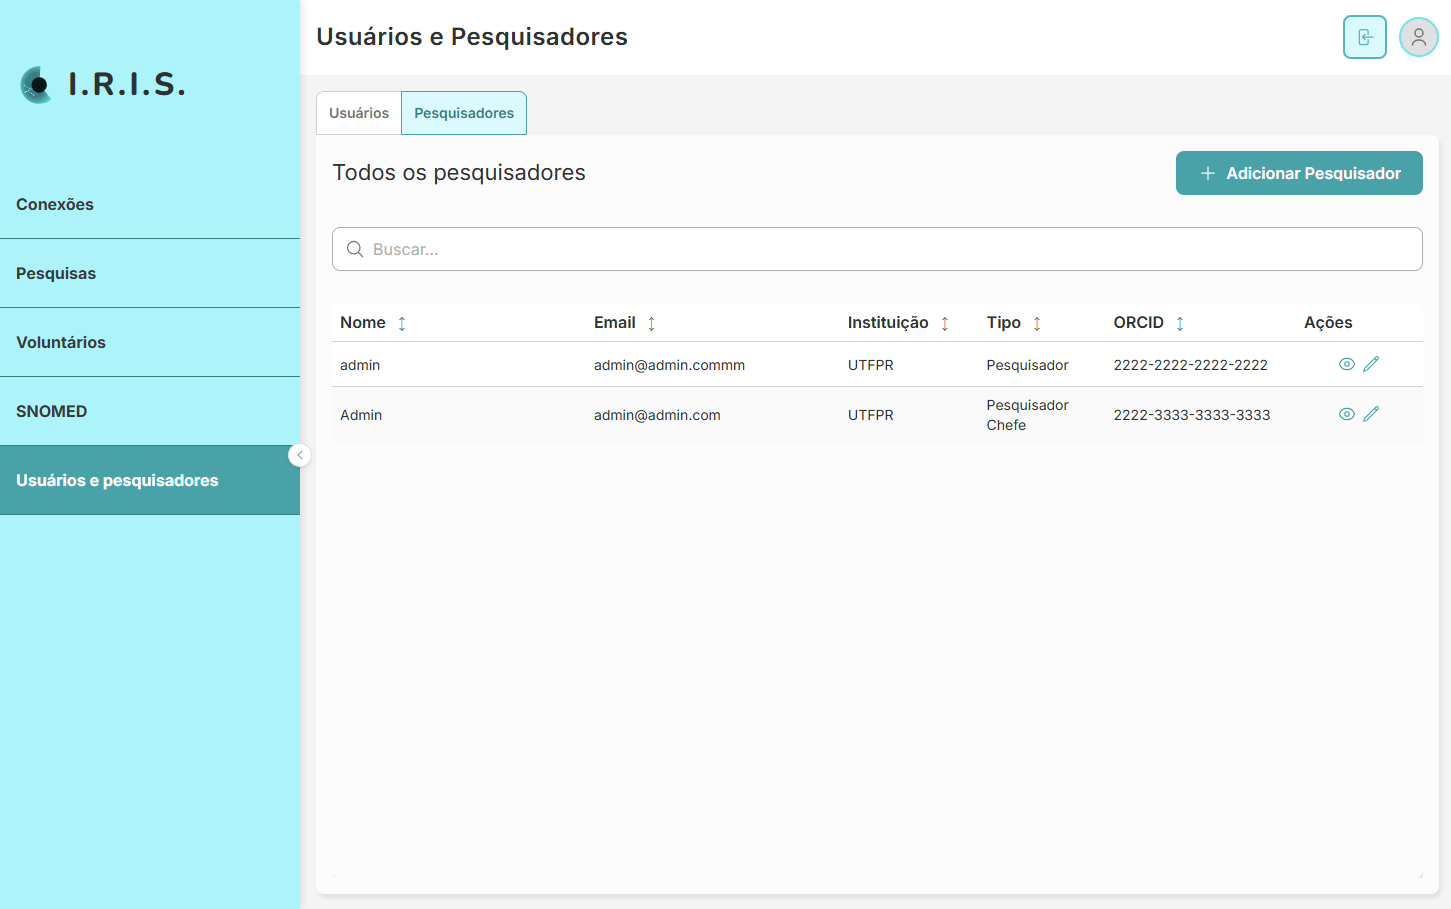
\includegraphics[scale=0.30]{figuras/Desenvolvimento/IRIS/screens/gestao-acessos-pesquisadores.png}
}
\fonte{}
\end{figure}

\begin{figure}[htb]
\caption{Tela de gestão de rótulos do IRIS \emph{web}, organizada em quatro abas correspondentes às entidades SNOMED CT manipuladas pelo NPI: (a) \emph{Região do Corpo}, (b) \emph{Estrutura do corpo}, (c) \emph{Modificador topográfico}, (d) \emph{Condição clínica}.}
\label{fig:irisTelaRotulos}
\centering
\subfloat[Aba \emph{Região do Corpo}]{
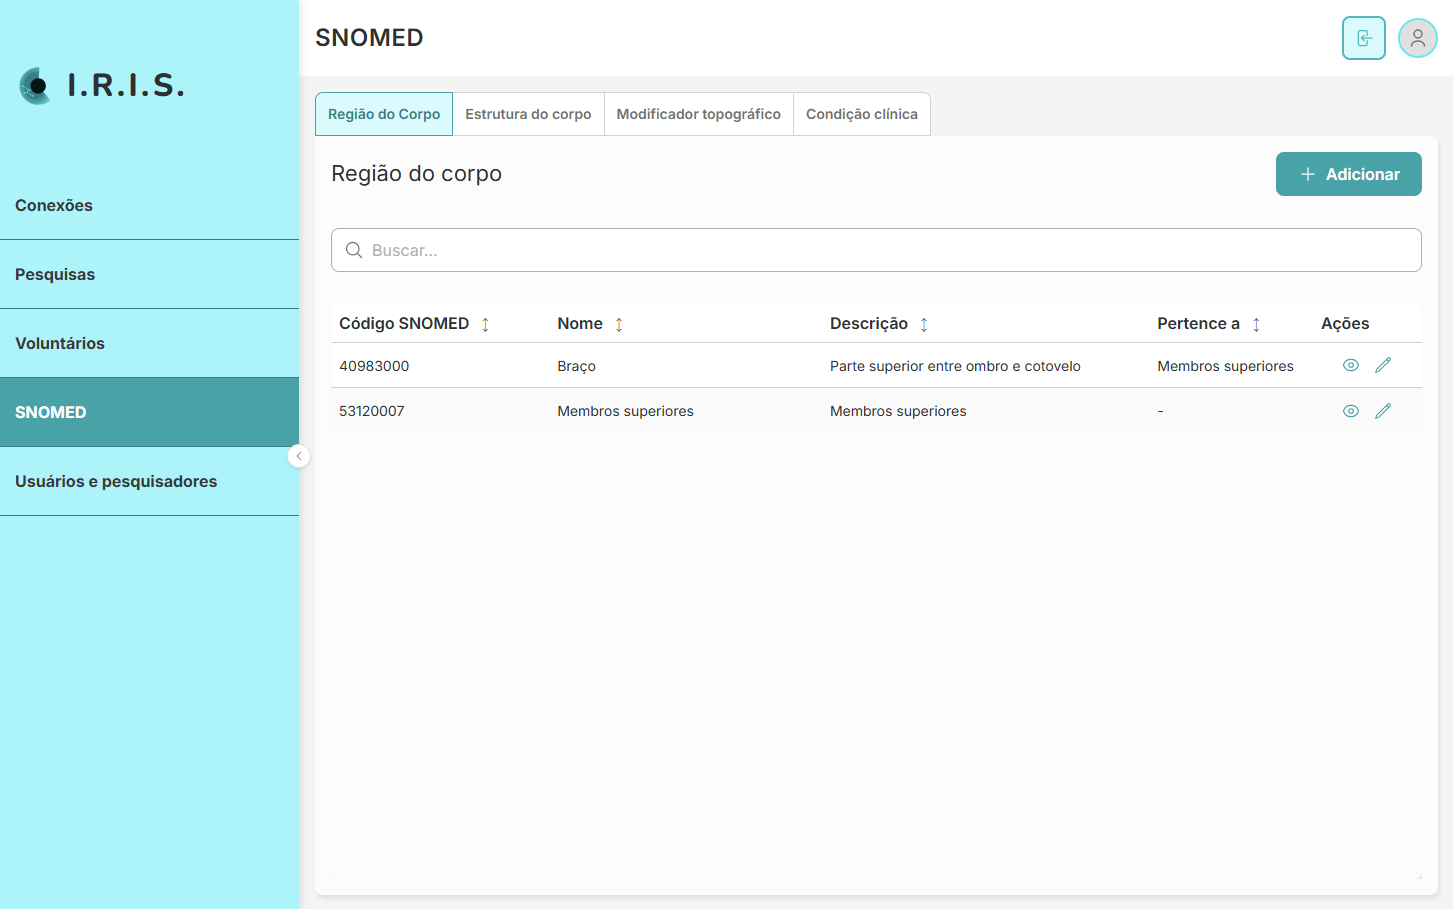
\includegraphics[scale=0.18]{figuras/Desenvolvimento/IRIS/screens/snomed-body-region.png}
}
\subfloat[Aba \emph{Estrutura do corpo}]{
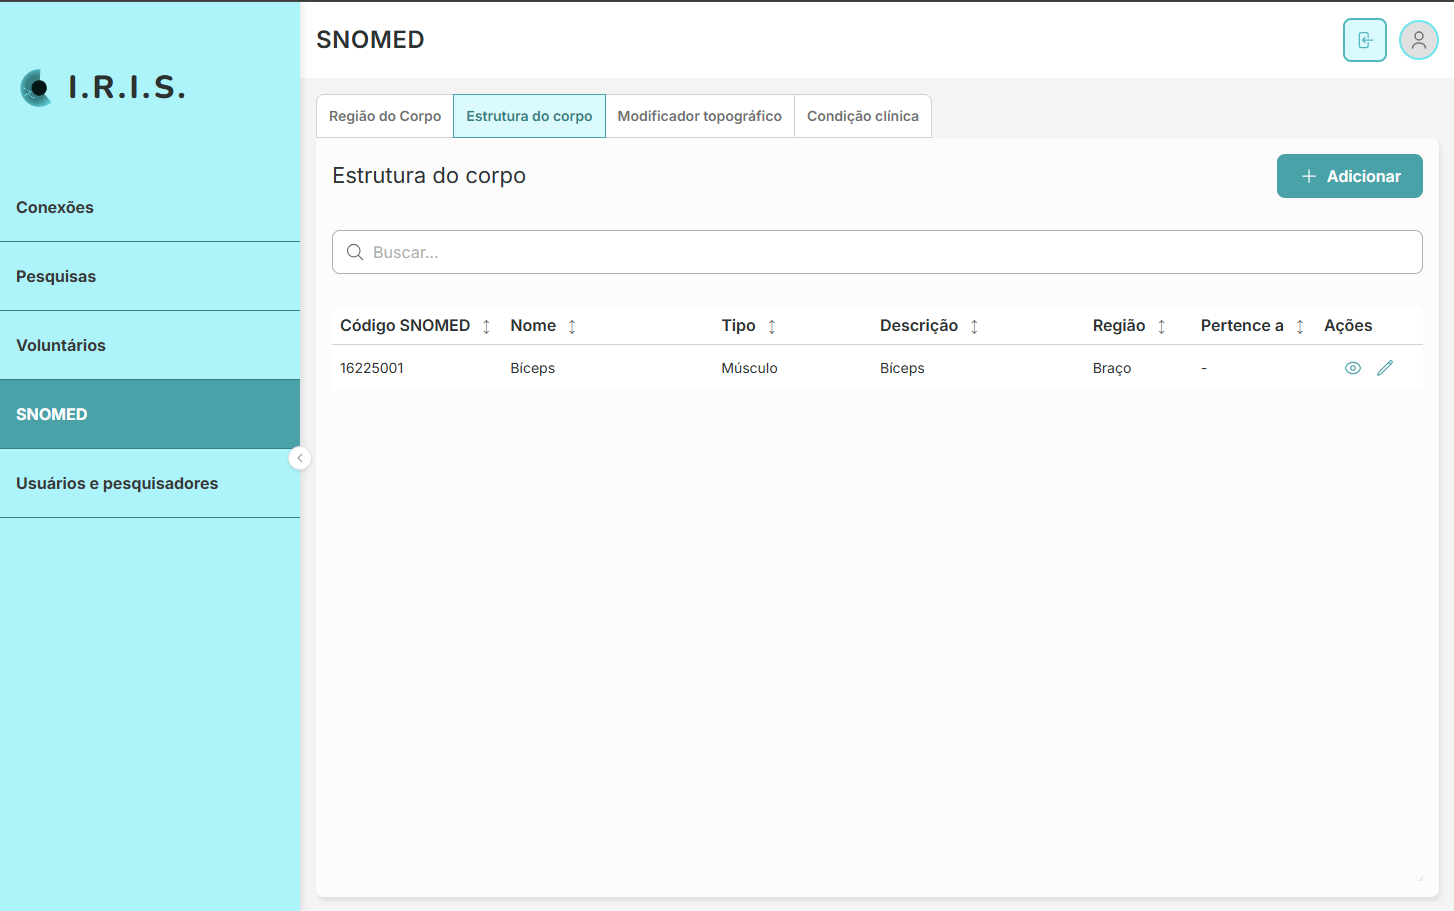
\includegraphics[scale=0.18]{figuras/Desenvolvimento/IRIS/screens/snomed-body-structure.png}
} \newline
\subfloat[Aba \emph{Modificador topográfico}]{
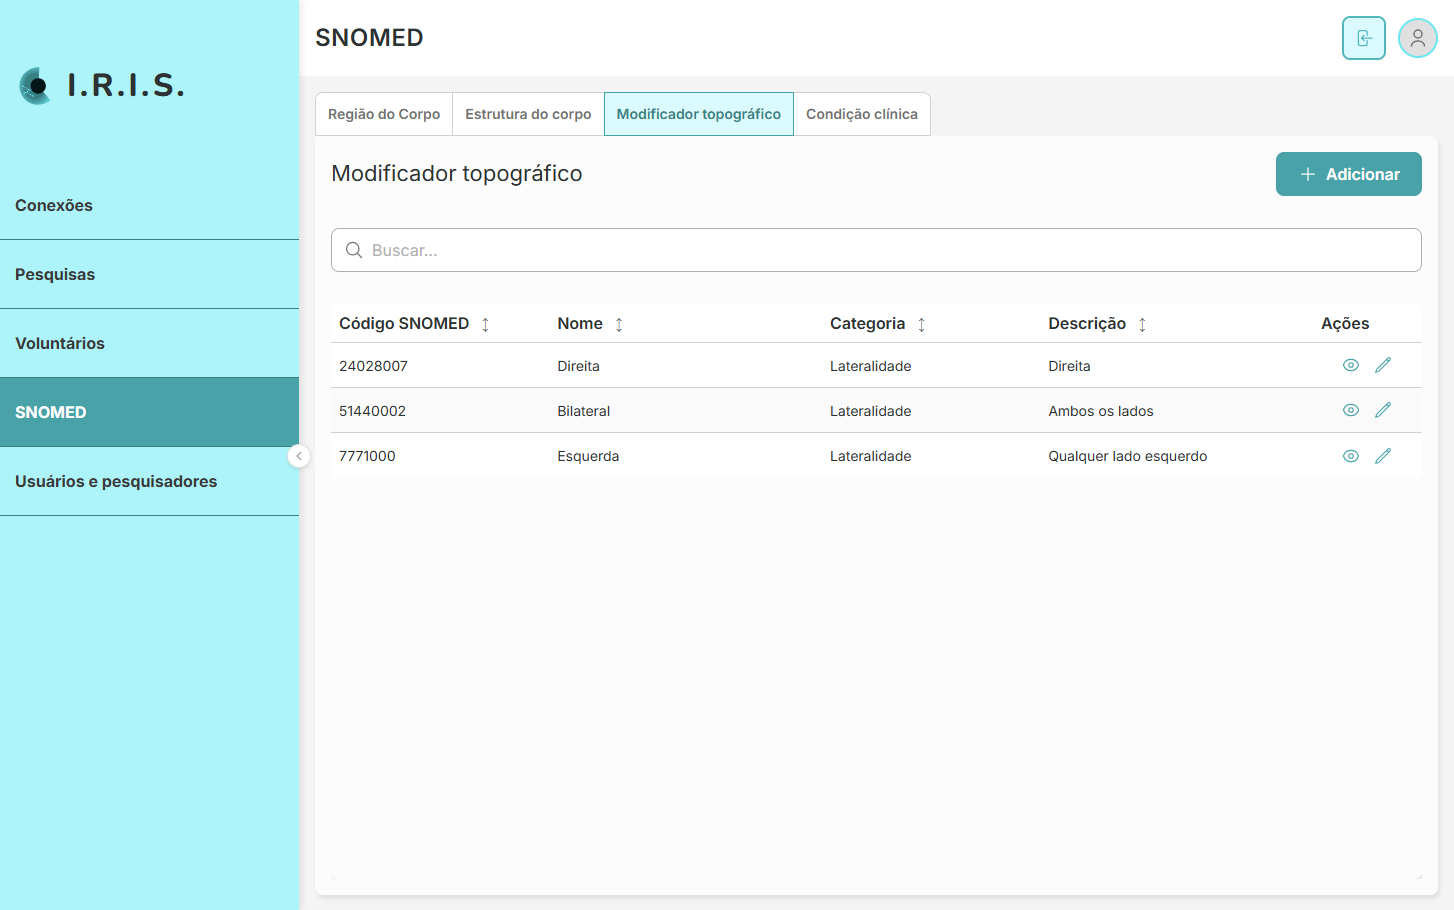
\includegraphics[scale=0.18]{figuras/Desenvolvimento/IRIS/screens/snomed-topografical-modifier.png}
}
\subfloat[Aba \emph{Condição clínica}]{
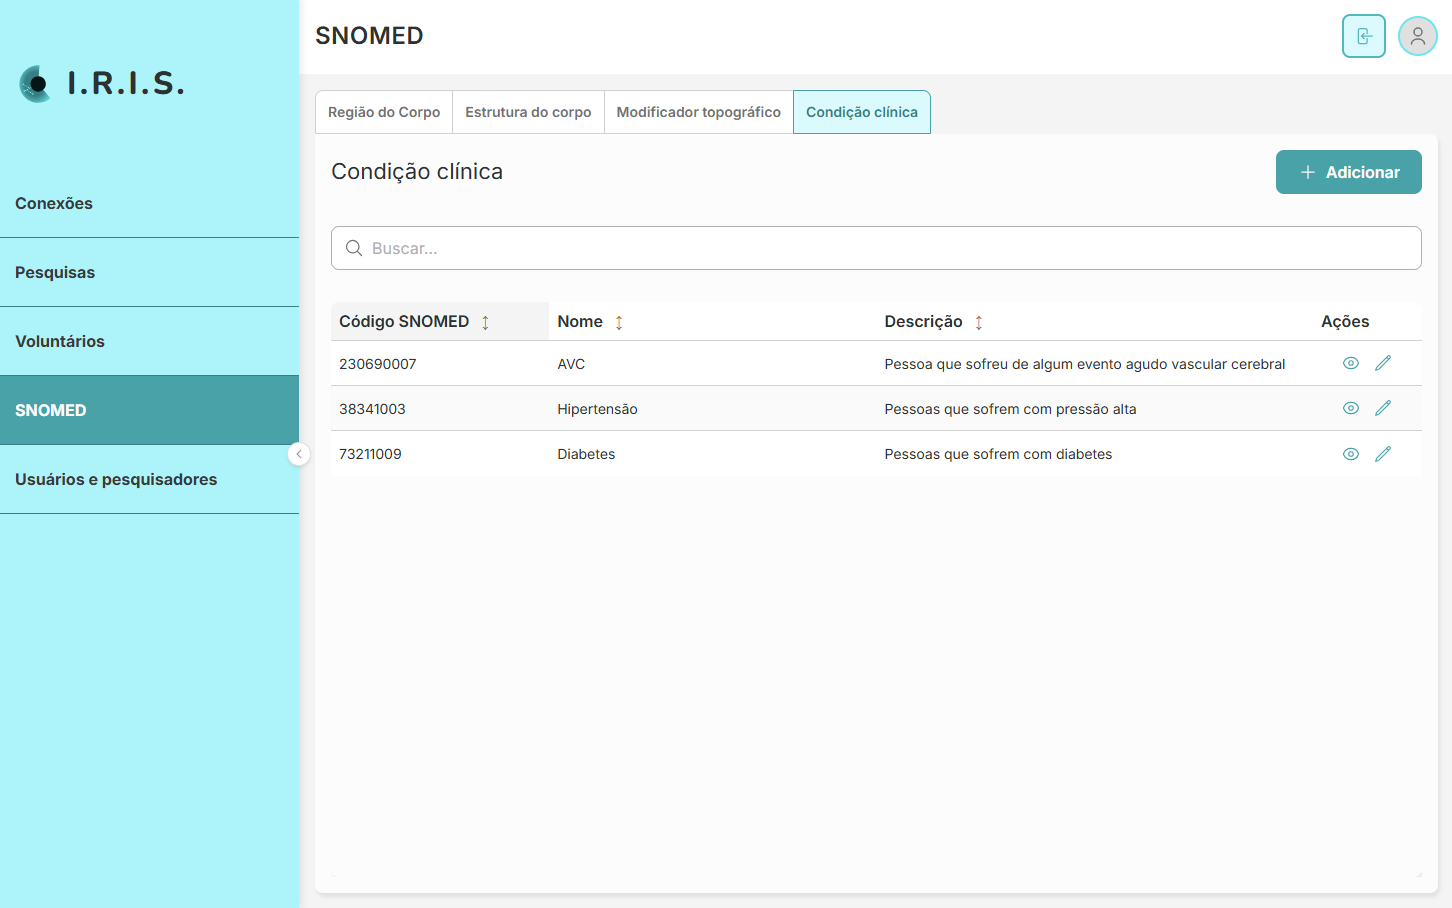
\includegraphics[scale=0.18]{figuras/Desenvolvimento/IRIS/screens/snomed-medical-condition.png}
}\hspace{0.15cm}
\fonte{}
\end{figure}

A consistência do sistema de \textit{design} é igualmente visível na tela de voluntários (Figura~\ref{fig:irisTelaPacientes}), que reaproveita o mesmo padrão de listagem das telas anteriores e introduz, na coluna \emph{Consentimento}, a primeira ocorrência do padrão visual de \emph{etiquetas coloridas} usado pelo IRIS \emph{web} para sinalizar estados discretos com alta carga informacional --- nesse caso, indicando se o voluntário concedeu autorização para a participação na pesquisa. O cadastro de um novo voluntário (Figura~\ref{fig:irisTelaPacientes}-b), por sua vez, materializa em formulário o conjunto de atributos clínicos e administrativos previstos para a entidade: dados de identificação (nome completo, e-mail, data de nascimento, gênero), código pseudonimizado derivado do CPF, atributos antropométricos opcionais (altura, peso, tipo sanguíneo), \emph{status} de consentimento e a possibilidade de associar condições médicas codificadas em SNOMED CT à ficha do participante. A tela de detalhes de um projeto de pesquisa (Figura~\ref{fig:irisTelaPesquisas}-b) é a única que se afasta do padrão de listagem plana, por ser também a expressão mais visível da hierarquia de coletas: cada subentidade ocupa uma aba dedicada (\emph{Pesquisadores}, \emph{Voluntários}, \emph{Aplicações}, \emph{Dispositivos} e \emph{Sensores}), acompanhada de contador entre parênteses, o que permite ao pesquisador editar separadamente cada conjunto associado ao projeto. A tela disponibiliza ainda um botão \emph{Exportar} no canto superior direito, que reúne, em um único arquivo, os metadados da hierarquia e as gravações vinculadas às sessões de coleta. Já a listagem de projetos (Figura~\ref{fig:irisTelaPesquisas}-a) repete o padrão de \emph{etiqueta colorida} no \emph{status} do projeto e oferece, em linha, uma ação adicional de exportação rápida ao lado das ações usuais de visualização e edição.

\begin{figure}[htb]
\caption{Telas de gestão de voluntários do IRIS \emph{web}: (a) voluntários cadastrados, (b) cadastro de novo voluntário.}
\label{fig:irisTelaPacientes}
\centering
\subfloat[Voluntários cadastrados]{
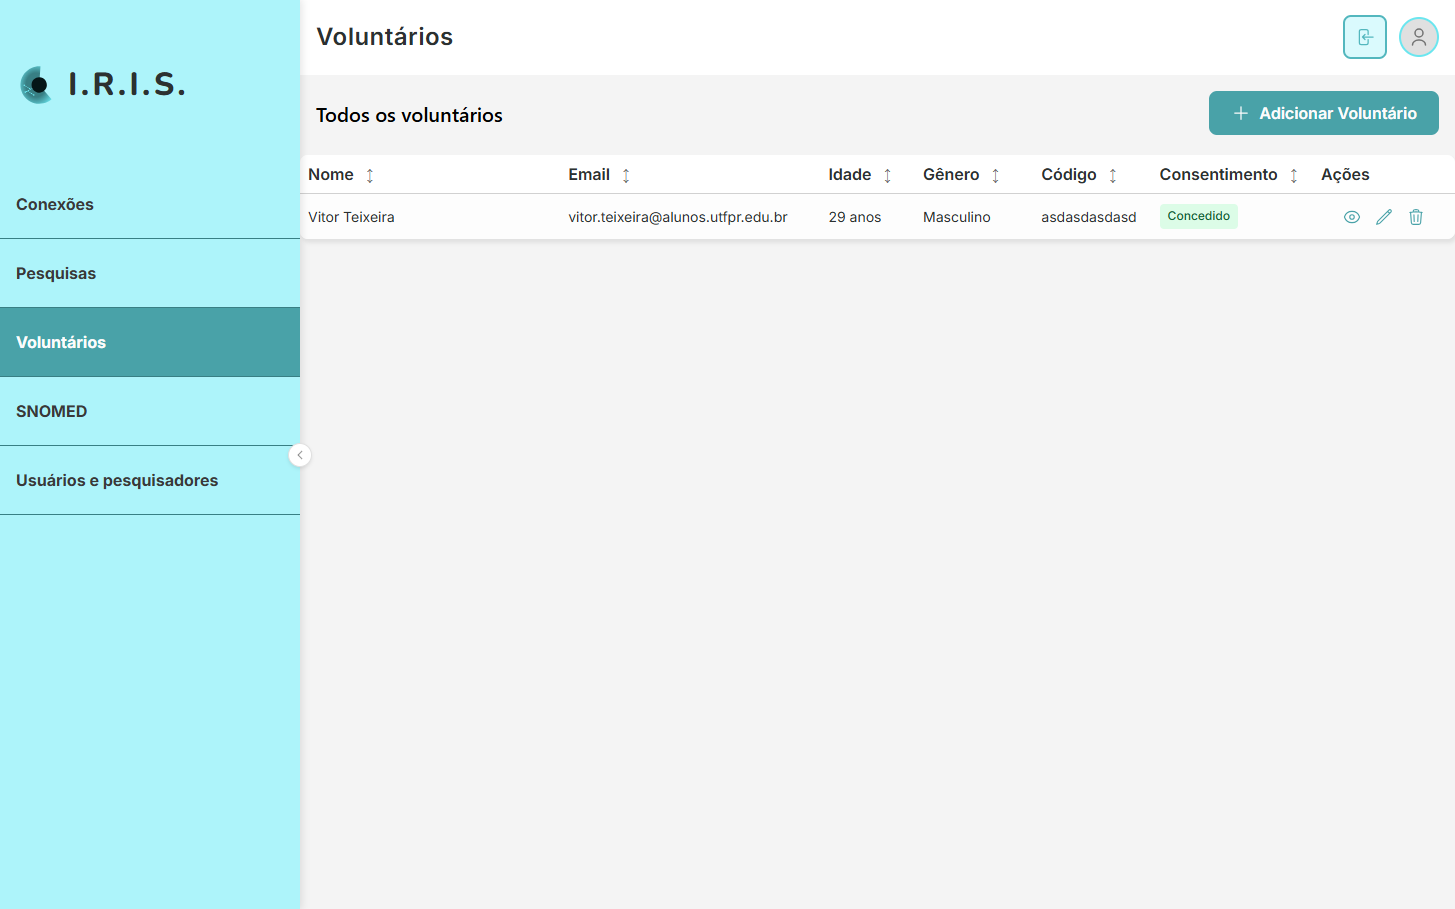
\includegraphics[scale=0.30]{figuras/Desenvolvimento/IRIS/screens/voluntarios-lista.png}
}\hspace{0.15cm}
\subfloat[Novo voluntário]{
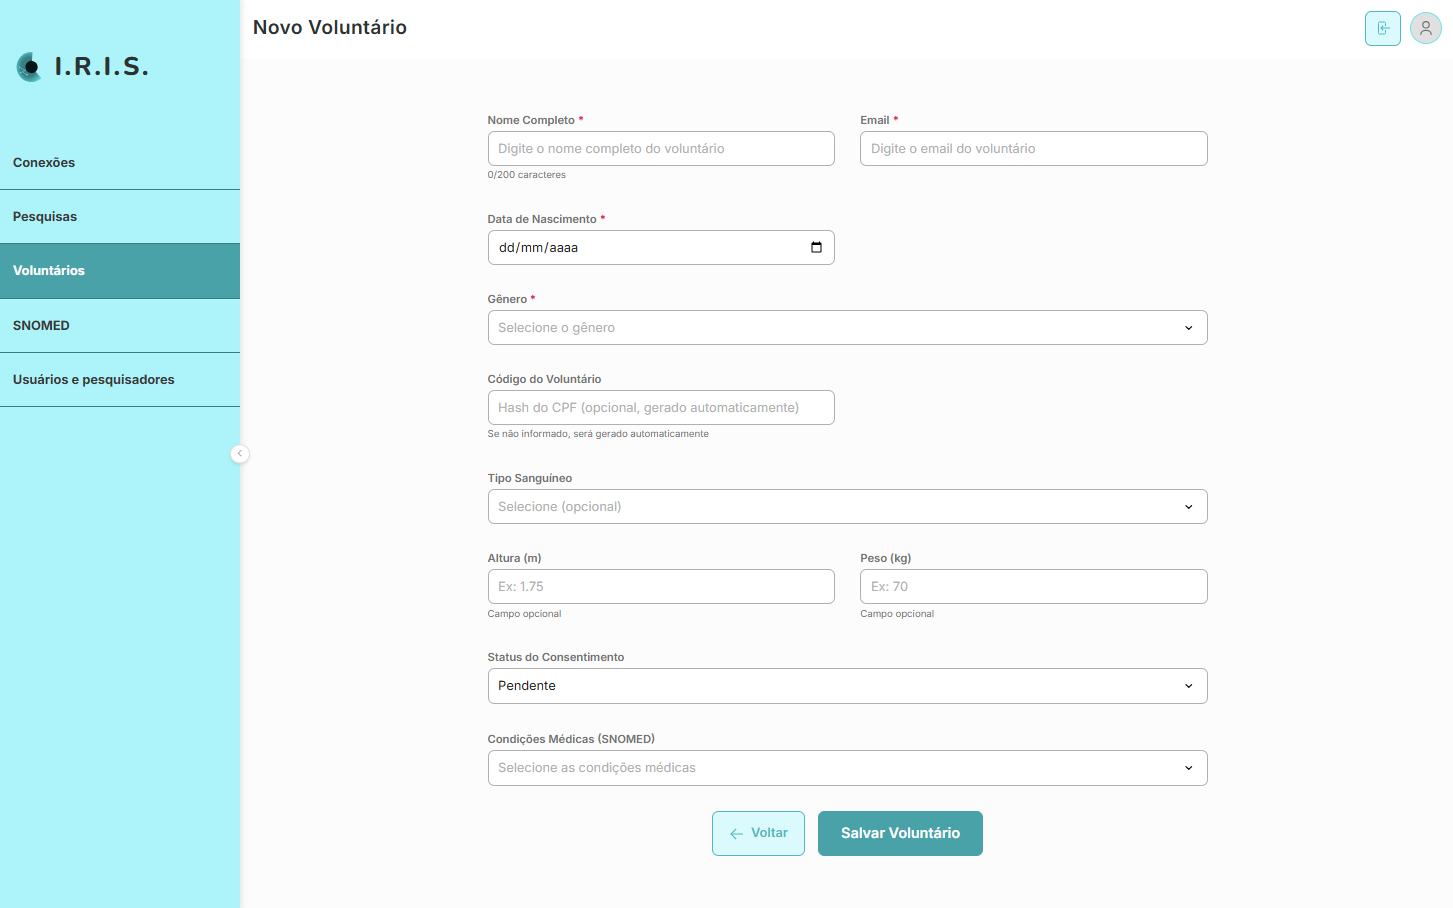
\includegraphics[scale=0.35]{figuras/Desenvolvimento/IRIS/screens/voluntarios-novo.png}
}
\fonte{}
\end{figure}

\begin{figure}[htb]
\caption{Telas de gestão de pesquisas do IRIS \emph{web}: (a) pesquisas cadastradas, (b) detalhes da pesquisa.}
\label{fig:irisTelaPesquisas}
\centering
\subfloat[Pesquisas cadastradas]{
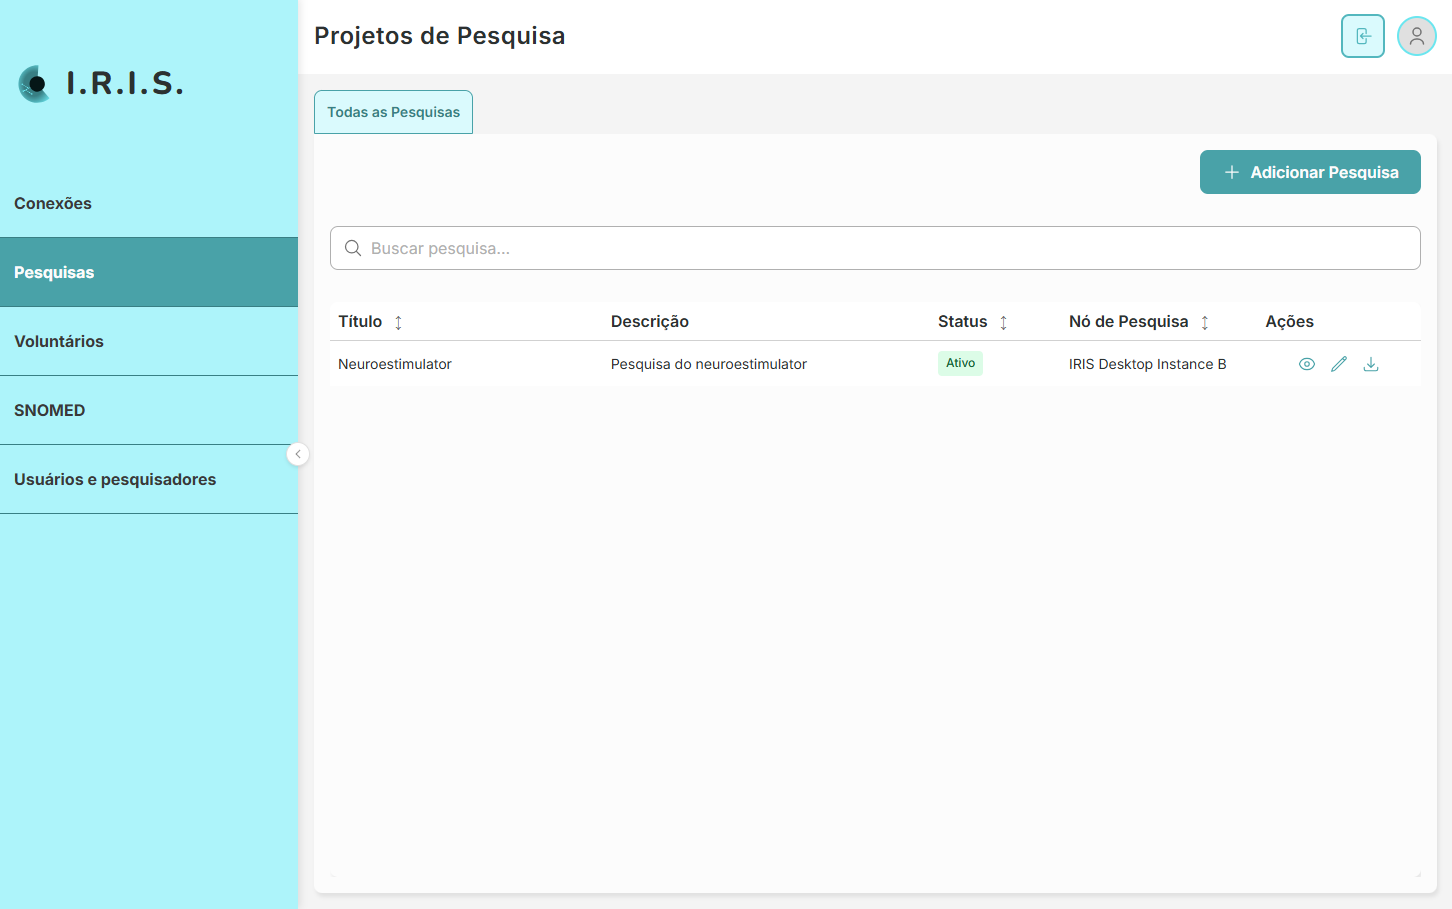
\includegraphics[scale=0.30]{figuras/Desenvolvimento/IRIS/screens/pesquisa-lista.png}
}\hspace{0.15cm}
\subfloat[Detalhes da pesquisa]{
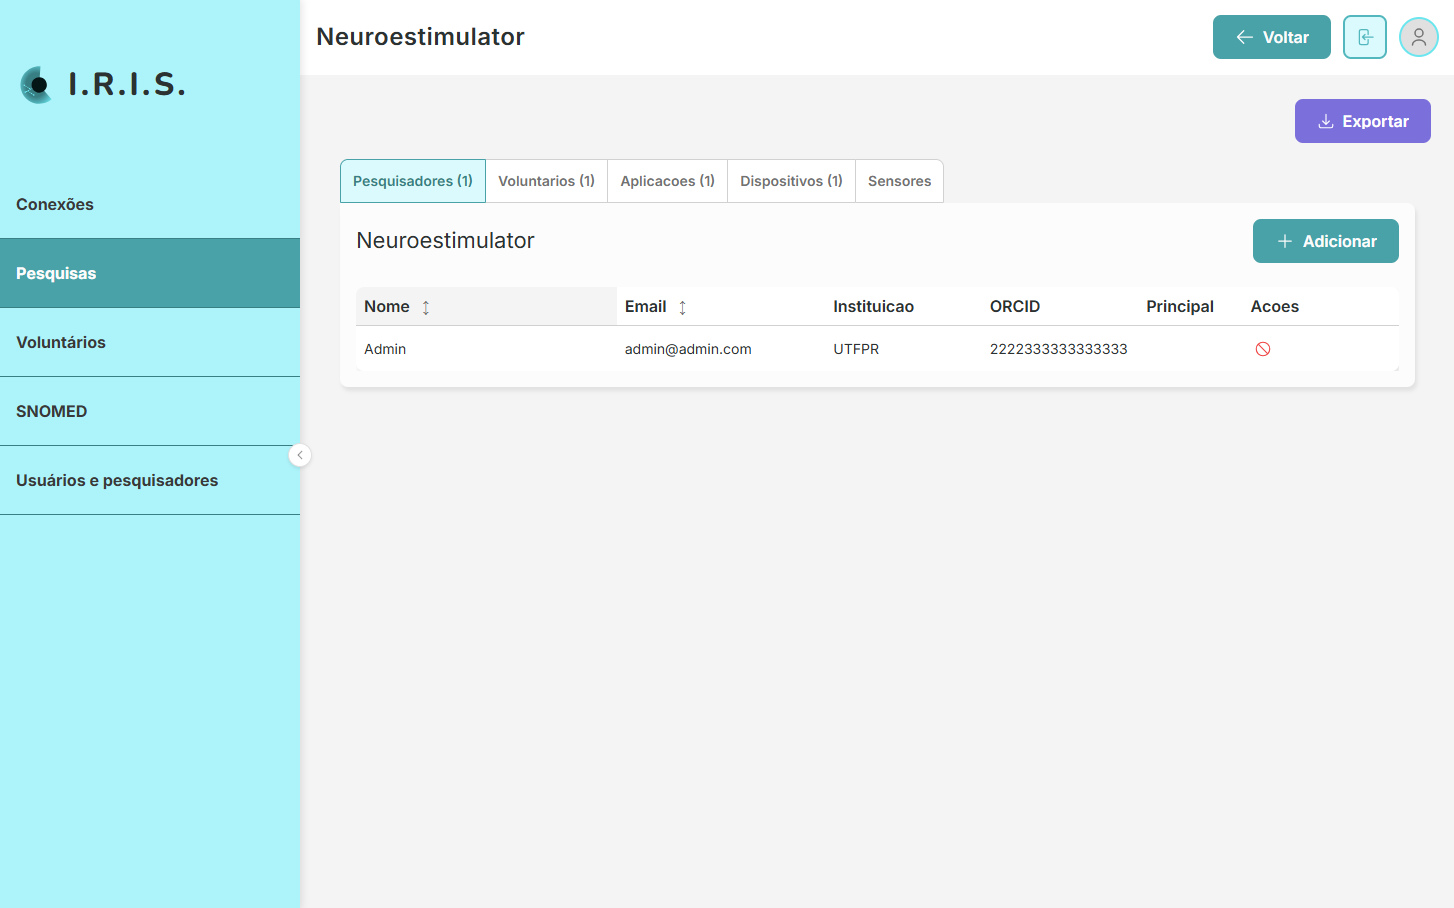
\includegraphics[scale=0.30]{figuras/Desenvolvimento/IRIS/screens/pesquisa-detalhes.png}
}
\fonte{}
\end{figure}

A última tela de operação corrente é a de conexões federadas (Figura~\ref{fig:irisTelaConexoesAtivas}), que traduz a máquina de estados apresentada na Subseção~\ref{subsubsec:IRISFederacao} em um par de abas (\emph{Todas as conexões} e \emph{Solicitações}) que separam visualmente as conexões já autorizadas das que aguardam decisão. A coluna \emph{Last Sync} apresenta o tempo decorrido em formato relativo (\textit{e.g.}, ``\emph{Synced 26d ago}'' ou ``\emph{Never}'' para conexões nunca sincronizadas), reforçando que a sincronização é uma operação intermitente e que sua atualidade é informação relevante para que o usuário decida se uma nova sincronização é necessária. Cada linha disponibiliza, além das ações usuais de visualização e edição, um ícone dedicado para disparar a sincronização com o nó correspondente. Acionada a partir desse ícone, a sincronização propriamente dita é acompanhada pelo \texttt{SyncProgressModal} (Figura~\ref{fig:irisTelaModalSync}), interface em três estados sequenciais: o manifesto inicial, em que o usuário confirma a operação após visualizar a contagem de entidades a transferir, discriminada por categoria (\emph{SNOMED}, \emph{Devices}, \emph{Sensors}, \emph{Volunteers}, \emph{Research}, \emph{Sessions} e \emph{Recordings}); o progresso, exibido enquanto o NPI local executa a transação atômica descrita na Subseção~\ref{subsubsec:IRISFederacao}; e o resumo final, que consolida o total de registros efetivamente transferidos e o horário de conclusão, fechando o ciclo iniciado pela pré-visualização.

\begin{figure}[htpb]
\captionsetup{width=0.8\textwidth}
\caption{Tela de conexões federadas do IRIS \emph{web}, exibida na aba \emph{Todas as conexões}, com o painel \emph{Conexões ativas} relacionando os nós já autorizados, seus respectivos níveis de acesso e o instante da última sincronização (coluna \emph{Last Sync}).}
\label{fig:irisTelaConexoesAtivas}
\centering
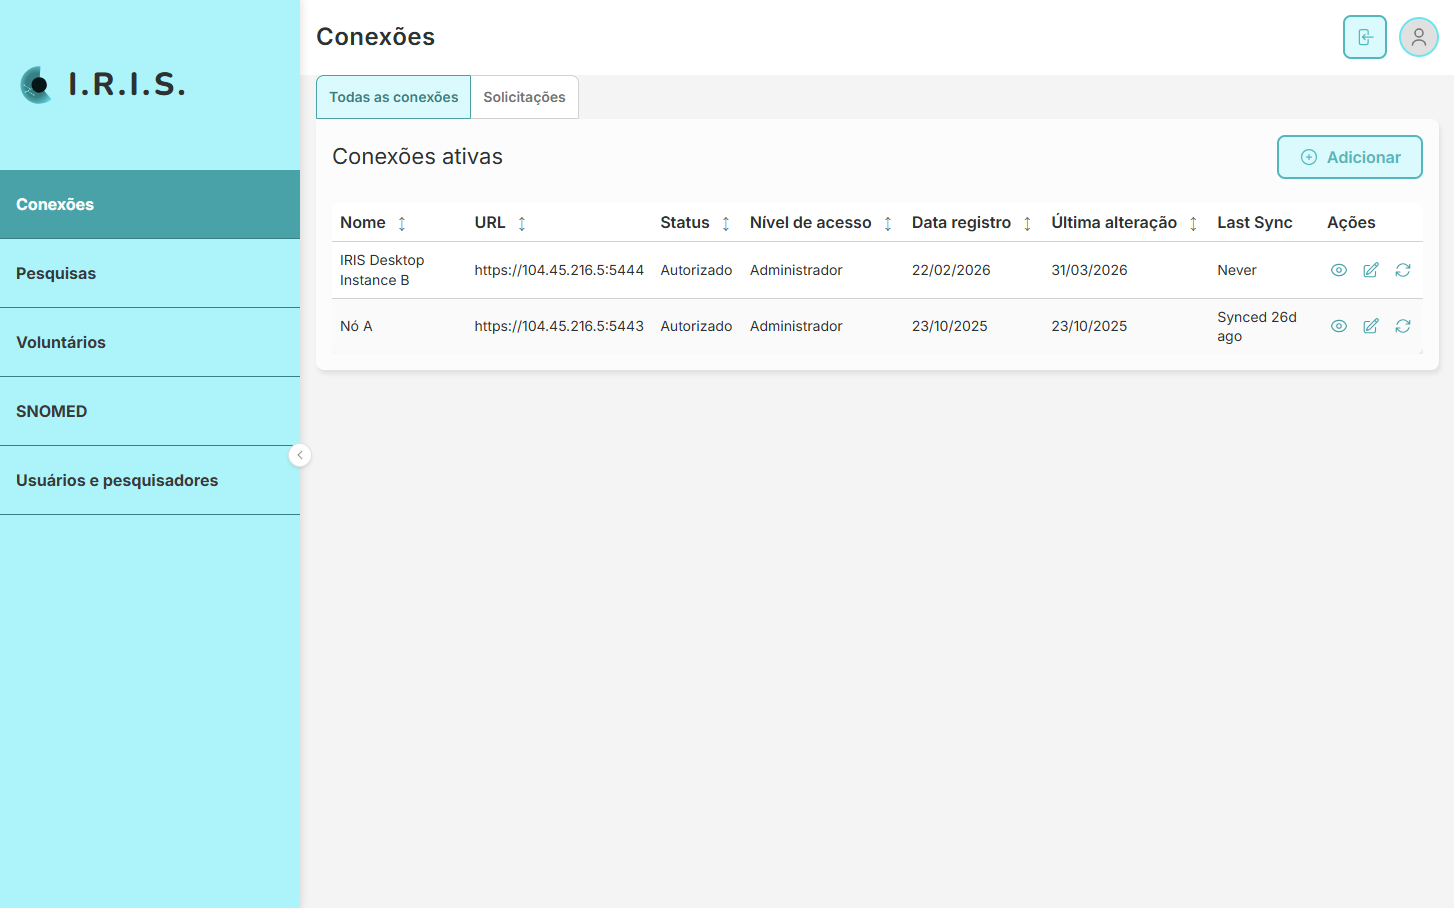
\includegraphics[scale=0.30]{figuras/Desenvolvimento/IRIS/screens/conexoes-lista.png}
\fonte{}
\end{figure}

\begin{figure}[htb]
\caption{Modal de sincronização do IRIS \emph{web}: (a) início da sincronização, (b) sincronização em progresso, (c) resumo final da sincronização.}
\label{fig:irisTelaModalSync}
\centering
\subfloat[Início da sincronização]{
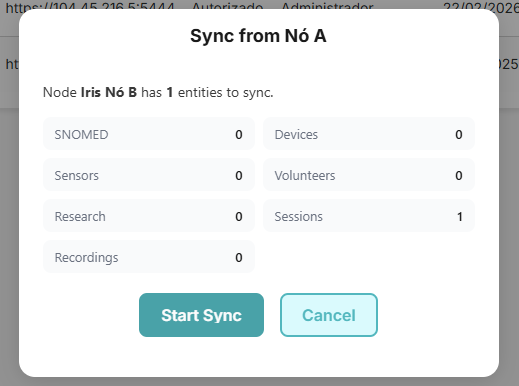
\includegraphics[scale=0.40]{figuras/Desenvolvimento/IRIS/screens/conexoes-sync.png}
}\hspace{0.15cm}
\subfloat[Sincronizando]{
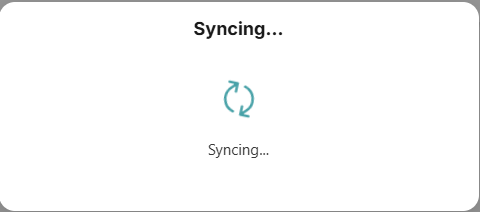
\includegraphics[scale=0.40]{figuras/Desenvolvimento/IRIS/screens/conexoes-syncing.png}
}\
\subfloat[Resumo da sincronização]{
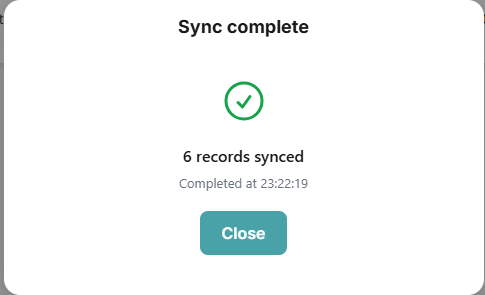
\includegraphics[scale=0.40]{figuras/Desenvolvimento/IRIS/screens/conexoes-sync-completed.png}
}
\fonte{}
\end{figure}

\newpage

% ----------------------------------------------------------------------
\section{Telas do IRIS \textit{Mobile}}\label{sec:apendiceTelasIRISMobile}
% ----------------------------------------------------------------------

Esta seção apresenta as cinco telas mais representativas do IRIS \textit{Mobile} (Subseção~\ref{subsec:IRISMobileTelas}), dispostas na ordem em que tipicamente são percorridas durante uma coleta: pareamento do dispositivo (Figura~\ref{fig:irisMobileTelaPareamento}), configuração da sessão clínica (Figura~\ref{fig:irisMobileTelaNewSession}), gerenciamento da sessão ativa (Figura~\ref{fig:irisMobileTelaSessaoAtiva}), captura ao vivo (Figura~\ref{fig:irisMobileTelaCaptura}) e, ao final, consulta ao histórico de coletas (Figura~\ref{fig:irisMobileTelaHistorico}).

A \texttt{BluetoothScreen} (Figura~\ref{fig:irisMobileTelaPareamento}) é o ponto de entrada do fluxo de coleta e ilustra o padrão de organização visual do aplicativo: cabeçalho com o título da seção e ação contextual de atualização da lista, agrupamento ``\textsc{Paired Devices}'' contendo os dispositivos previamente pareados ao sistema operacional e barra de navegação global persistente no rodapé (\emph{Home}, \emph{History}, \emph{Bluetooth}, \emph{Settings}), por meio da qual o usuário transita entre as demais telas do aplicativo.

\begin{figure}[htpb]
\caption{Tela de pareamento do IRIS \textit{Mobile}, com a listagem dos dispositivos pareados ao sistema operacional.}
\label{fig:irisMobileTelaPareamento}
\centering
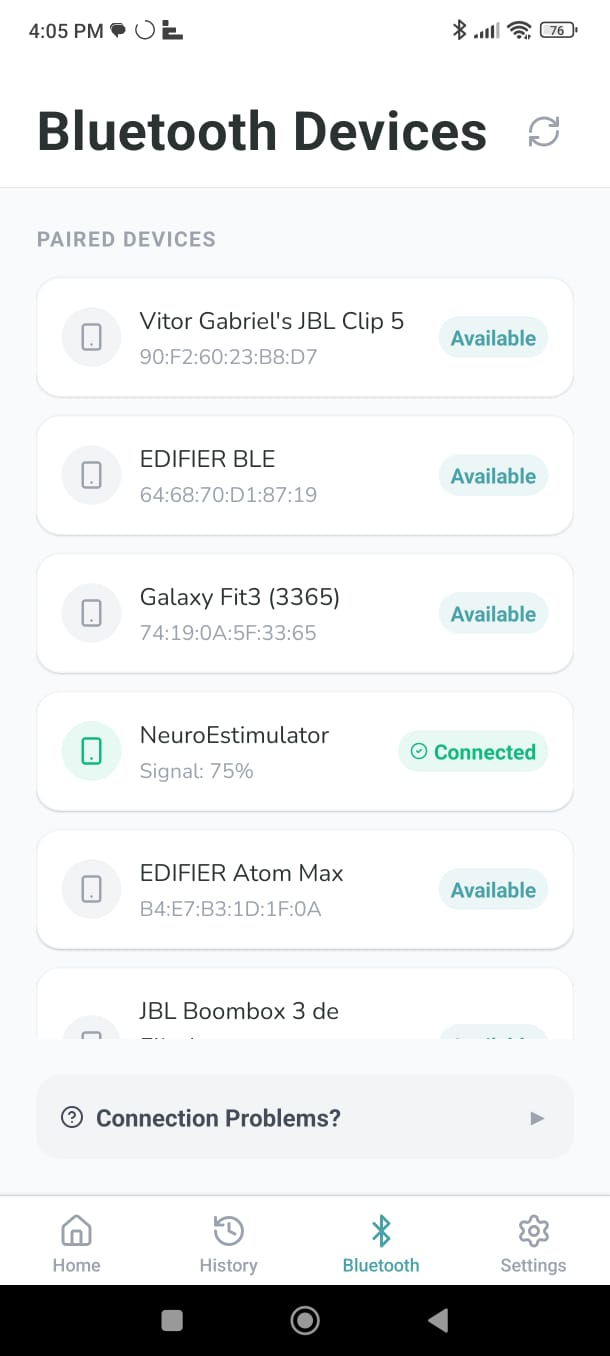
\includegraphics[scale=0.20]{figuras/telasIrisMobile/bluetoth_devices.jpeg}
\fonte{}
\end{figure}

A \texttt{SessionConfigScreen} (Figura~\ref{fig:irisMobileTelaNewSession}) é o local em que a sessão clínica recebe a contextualização semântica que distingue o IRIS \textit{Mobile} de um aplicativo genérico de captura de sinal. O formulário concentra a seleção do voluntário inscrito no projeto de pesquisa, da estrutura anatômica alvo da medição, dos modificadores topográficos aplicáveis --- todos extraídos do vocabulário SNOMED CT consumido por \texttt{SnomedService} (Subseção~\ref{subsec:IRISMobileArquitetura}) --- e do dispositivo e sensor que conduzirão a aquisição. Combinações frequentemente repetidas pelo pesquisador podem ser marcadas como configuração favorita; nesses casos, o \texttt{FavoriteRepository} grava localmente o conjunto completo de campos preenchidos, de modo que sessões posteriores possam ser pré-configuradas com um único toque.

\begin{figure}[htpb]
\caption{Tela de configuração de sessão do IRIS \textit{Mobile}, com a seleção de voluntário, estrutura anatômica alvo, modificadores topográficos, dispositivo e sensor no estado vazio (a) e (b), e preenchida com dados para sessão (c) e (d).}
\label{fig:irisMobileTelaNewSession}
\centering
\subfloat[Topo da tela vazio]{
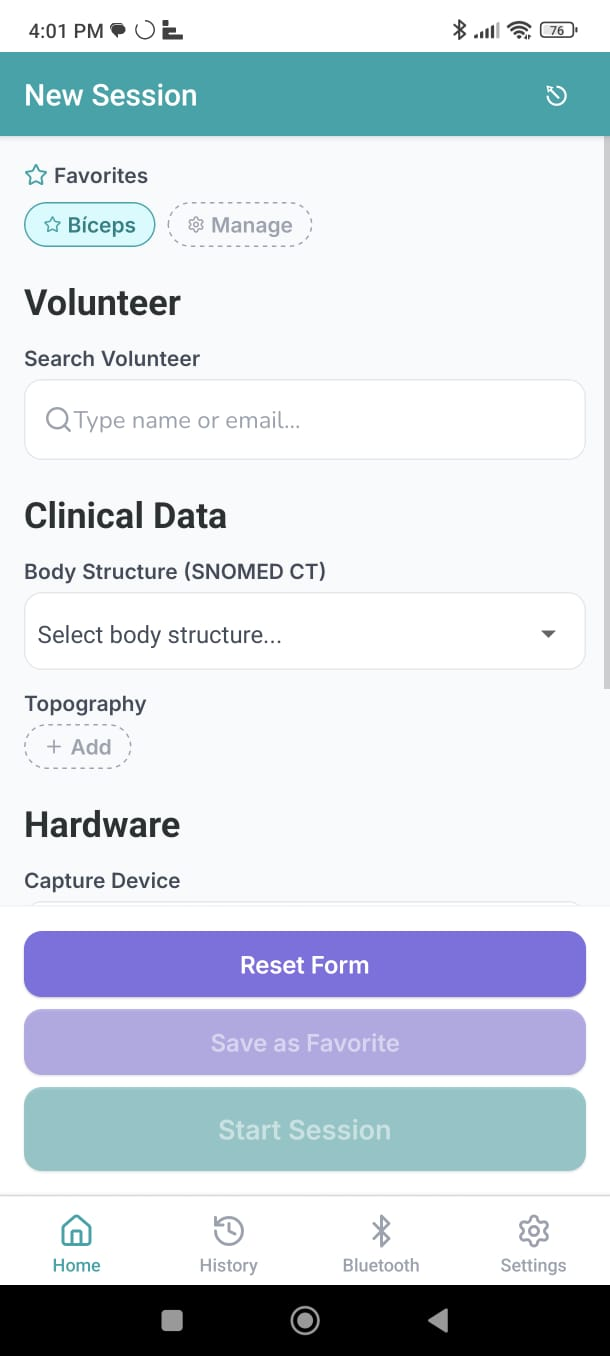
\includegraphics[scale=0.20]{figuras/telasIrisMobile/new_session_a.jpeg}
}\hspace{0.15cm}
\subfloat[Rodapé da tela vazio]{
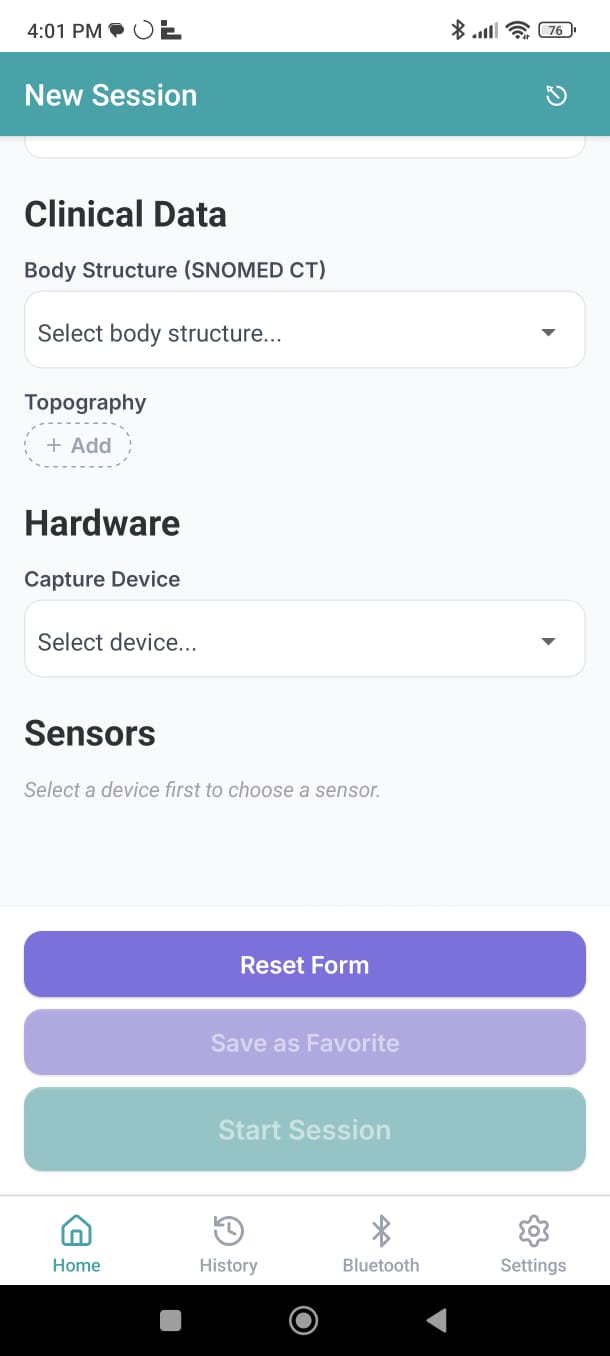
\includegraphics[scale=0.20]{figuras/telasIrisMobile/new_session_b.jpeg}
}\
\subfloat[Topo da tela preenchido]{
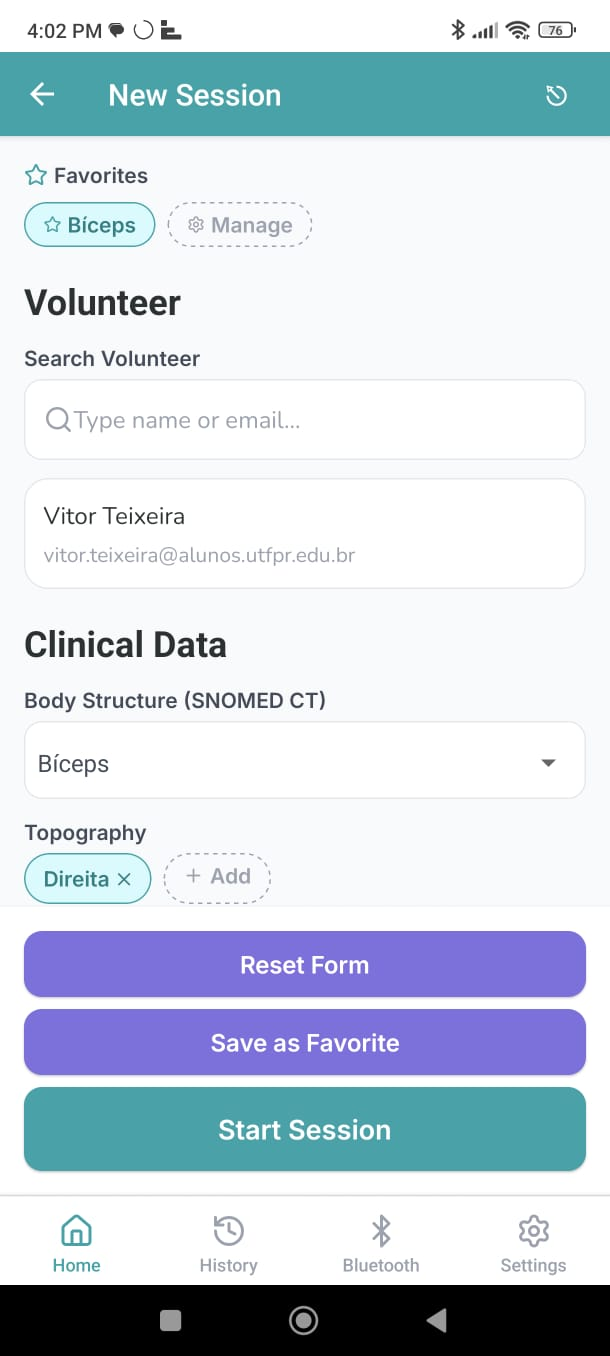
\includegraphics[scale=0.20]{figuras/telasIrisMobile/new_session_preenchida_a.jpeg}
}
\subfloat[Rodapé da tela preenchido]{
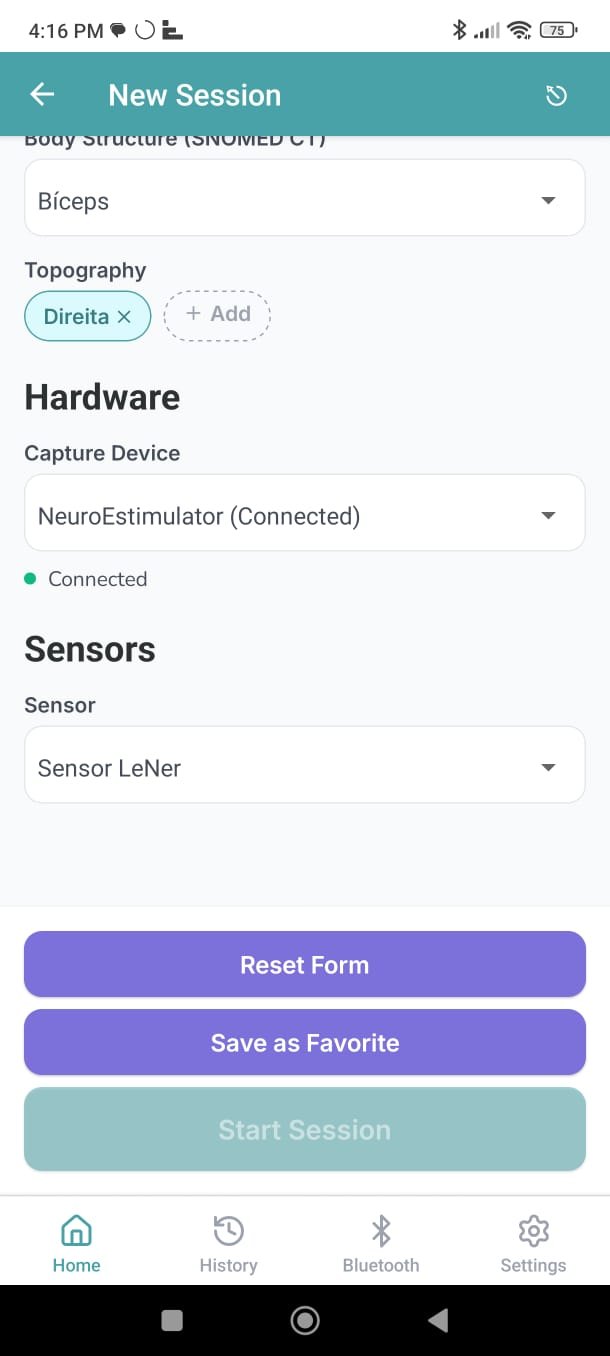
\includegraphics[scale=0.20]{figuras/telasIrisMobile/new_session_preenchida_b.jpeg}
}
\fonte{}
\end{figure}

A \texttt{ActiveSessionScreen} (Figura~\ref{fig:irisMobileTelaSessaoAtiva}-a) é a tela de coordenação da sessão clínica em curso. O cabeçalho exibe o título \emph{Active Session}, um cronômetro com a duração corrente da sessão e o nome do voluntário, seguido por um cartão de contexto que reapresenta a estrutura anatômica alvo e o dispositivo conectado. Na sequência, a área \textsc{Recordings} relaciona as gravações já produzidas, identificadas pelo \emph{timestamp} do arquivo CSV gerado e por uma etiqueta colorida indicativa do estado de sincronização daquela gravação (\textit{e.g.}, \emph{Pending}, em laranja). Um botão circular destacado dispara o início de uma nova gravação e, no rodapé do conteúdo, dois botões independentes encaminham o pesquisador para a \texttt{AnnotationsListScreen} (Figura~\ref{fig:irisMobileTelaSessaoAtiva}-b), onde gerencia as anotações associadas à sessão, ou para o encerramento explícito da coleta (\emph{End Session}). A separação entre essa tela e a \texttt{CaptureScreen} é uma decisão consciente: a sessão é a unidade que agrega as gravações e os rótulos discutidos na Subseção~\ref{subsec:IRISMobileRotulos}, enquanto a captura propriamente dita é uma operação pontual, repetível ao longo do tempo de duração da sessão.

\begin{figure}[htpb]
\caption{Telas associadas à sessão clínica em curso no IRIS \textit{Mobile}: (a) tela de sessão ativa, com a listagem das gravações já produzidas e o botão de início de nova gravação; (b) tela de anotações da sessão, acessível a partir da sessão ativa.}
\label{fig:irisMobileTelaSessaoAtiva}
\centering
\subfloat[Sessão Ativa]{
    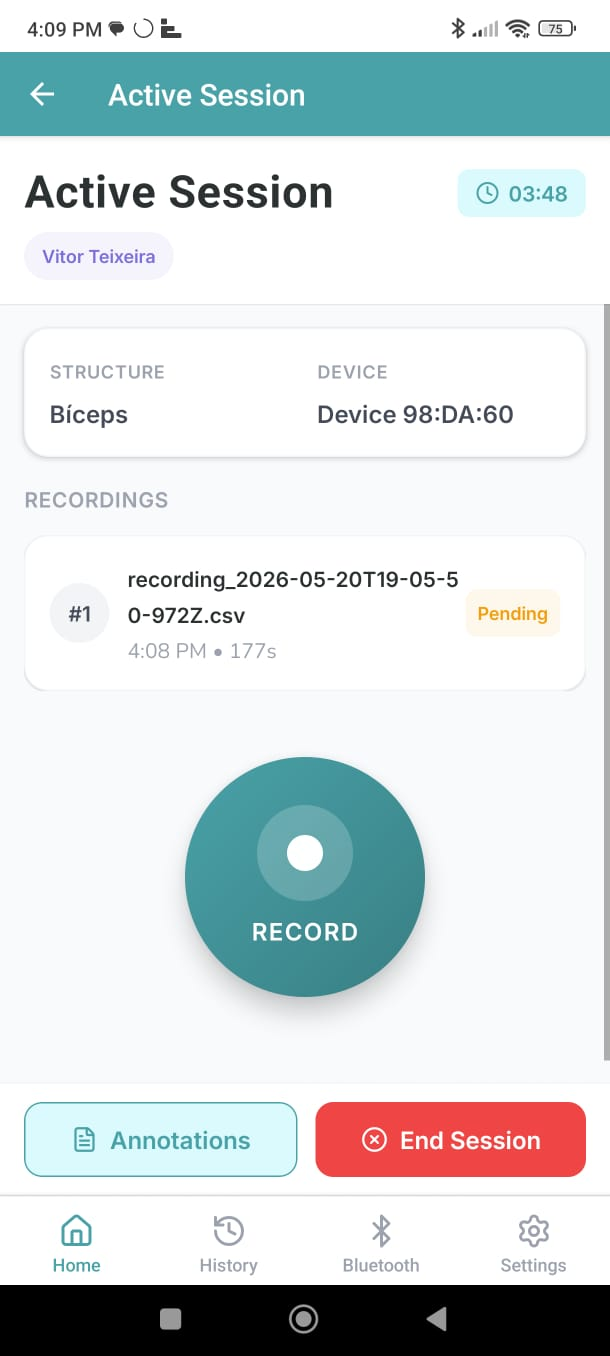
\includegraphics[scale=0.20]{figuras/telasIrisMobile/sessao_ativa.jpeg}
}
\subfloat[Anotações da Sessão]{
    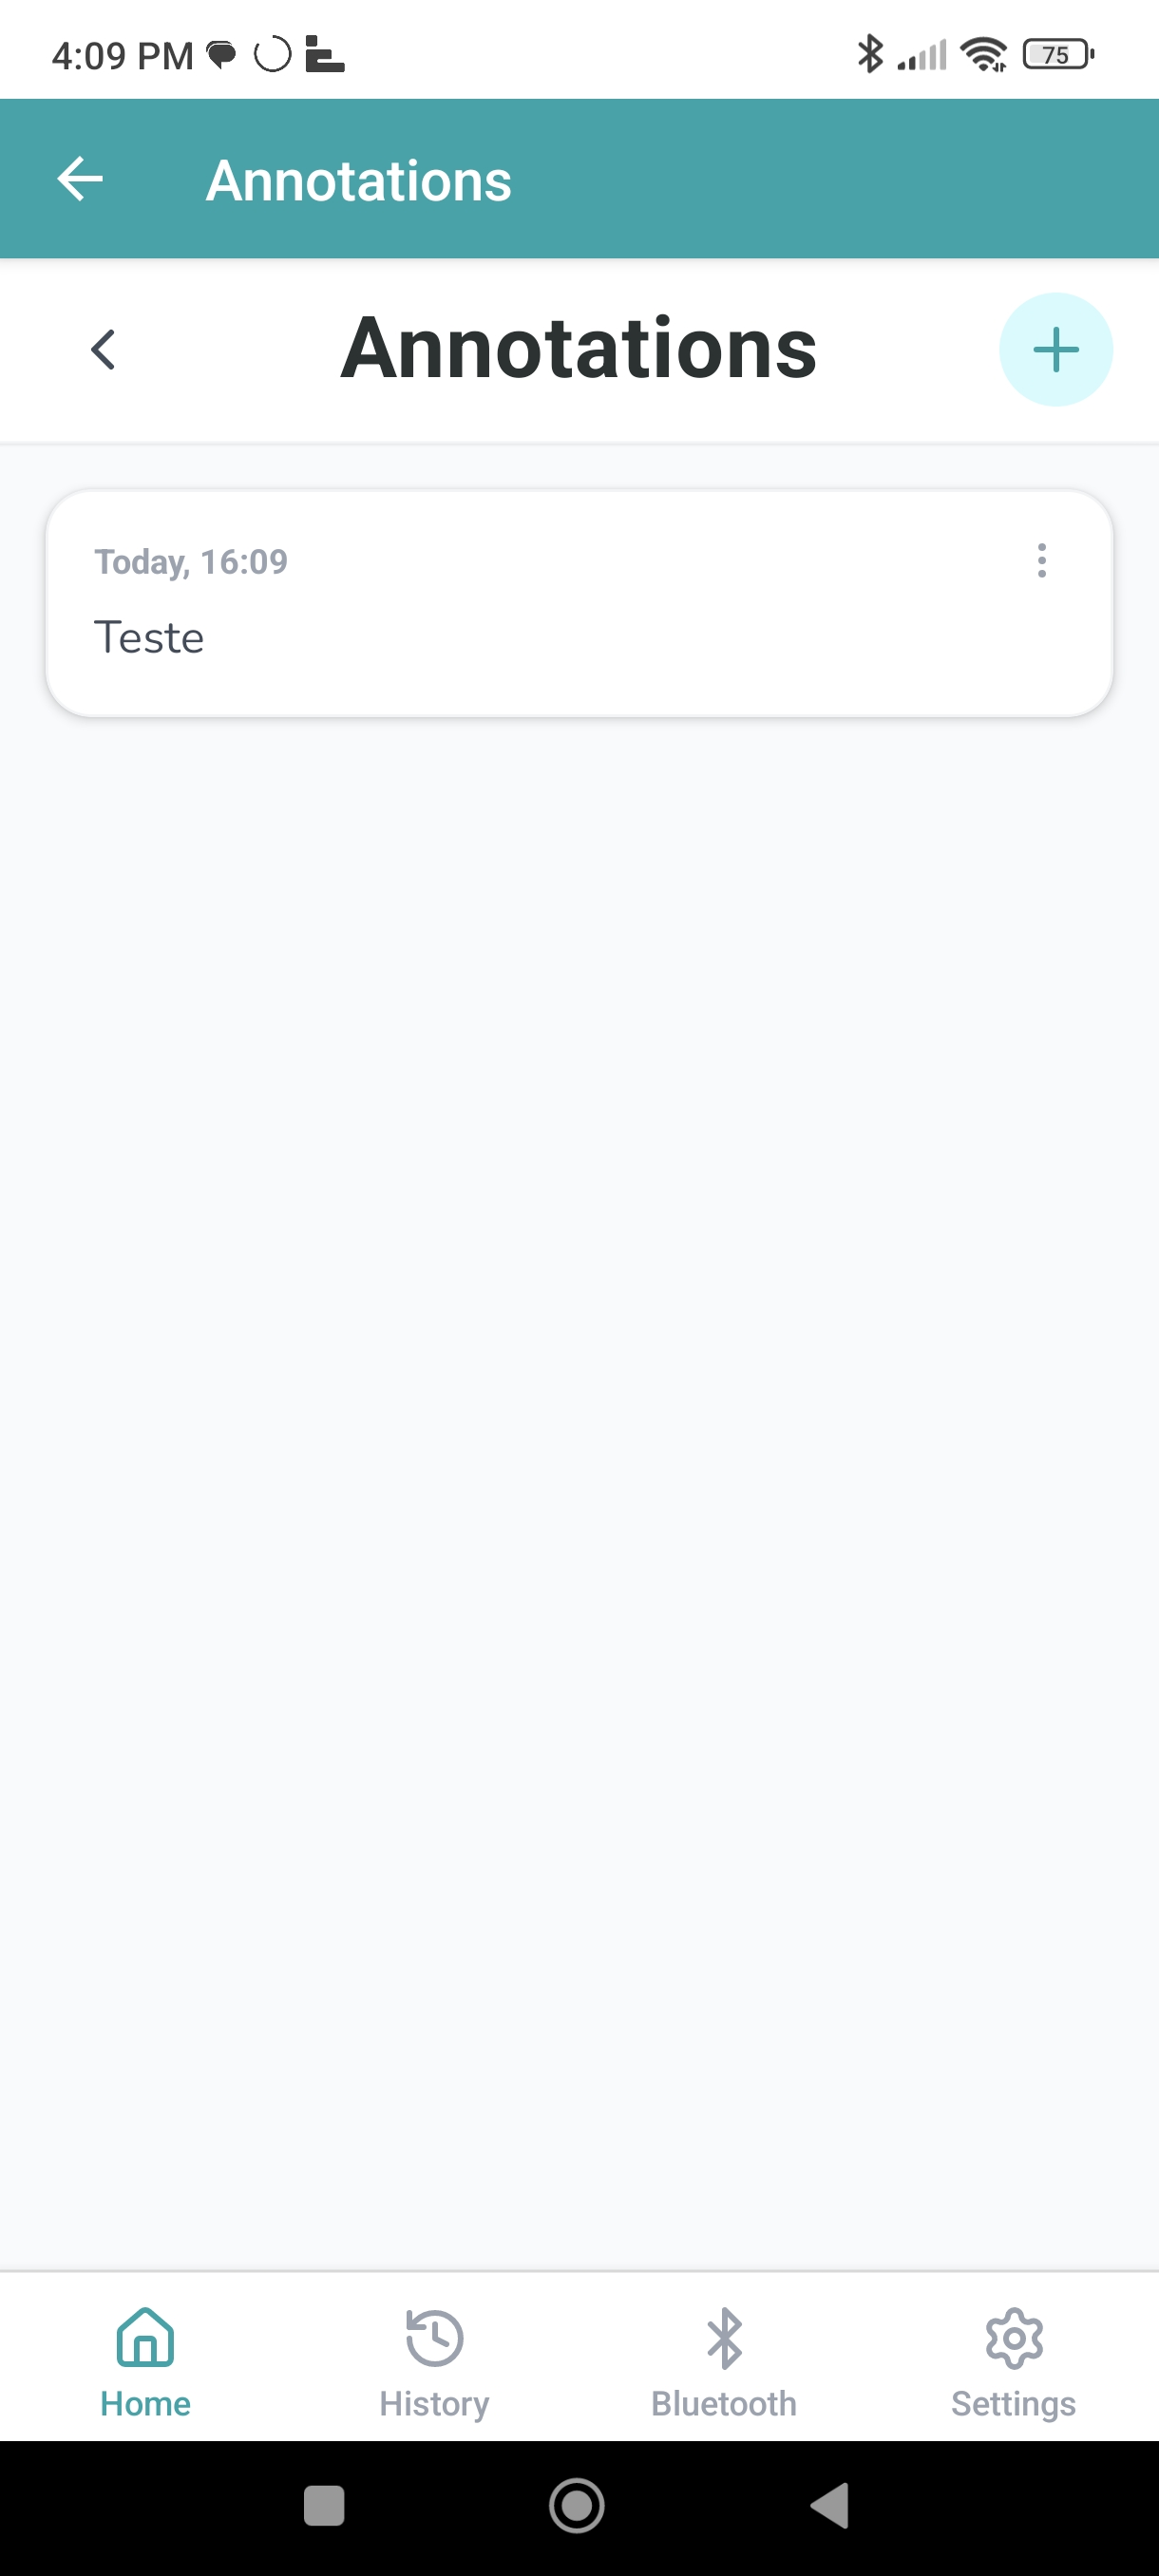
\includegraphics[scale=0.10]{figuras/telasIrisMobile/lista_anotacoes.jpeg}
}\
\fonte{}
\end{figure}

A \texttt{CaptureScreen} (Figura~\ref{fig:irisMobileTelaCaptura}) --- intitulada \emph{Data Capture} no cabeçalho --- é a tela operacional do aplicativo durante a aquisição. No topo, um indicador de gravação ativa e um cronômetro reportam o tempo decorrido desde o início da captura; abaixo deles, o gráfico em primeiro plano apresenta a janela móvel de quatro segundos do sinal sEMG filtrado, anotada com os parâmetros da renderização discutidos na Subseção~\ref{subsec:IRISMobileCaptura} (\emph{215~Hz}, \emph{Last 4s window}, \emph{40~Hz display}). Sob o gráfico, três cartões de telemetria condensam, em tempo real, o valor RMS em microvolts, a frequência de amostragem e um indicador qualitativo de qualidade de sinal; o conjunto se encerra com um botão dedicado e visualmente destacado de parada da gravação, suficiente para que o pesquisador concentre a atenção no participante e não na interface durante a coleta. A comparação entre o bíceps em repouso (a) e em contração voluntária (b) torna evidente, ainda, o aumento da amplitude do sinal e do valor RMS associado.

\begin{figure}[htpb]
\caption{Tela de captura ao vivo do IRIS \textit{Mobile}, com o gráfico do sinal sEMG filtrado, cartões de telemetria (RMS, frequência e qualidade de sinal) e controle de parada da gravação: (a) bíceps em repouso e (b) bíceps em contração voluntária.}
\label{fig:irisMobileTelaCaptura}
\centering
\subfloat[Gráfico do sinal sEMG bíceps em repouso]{
    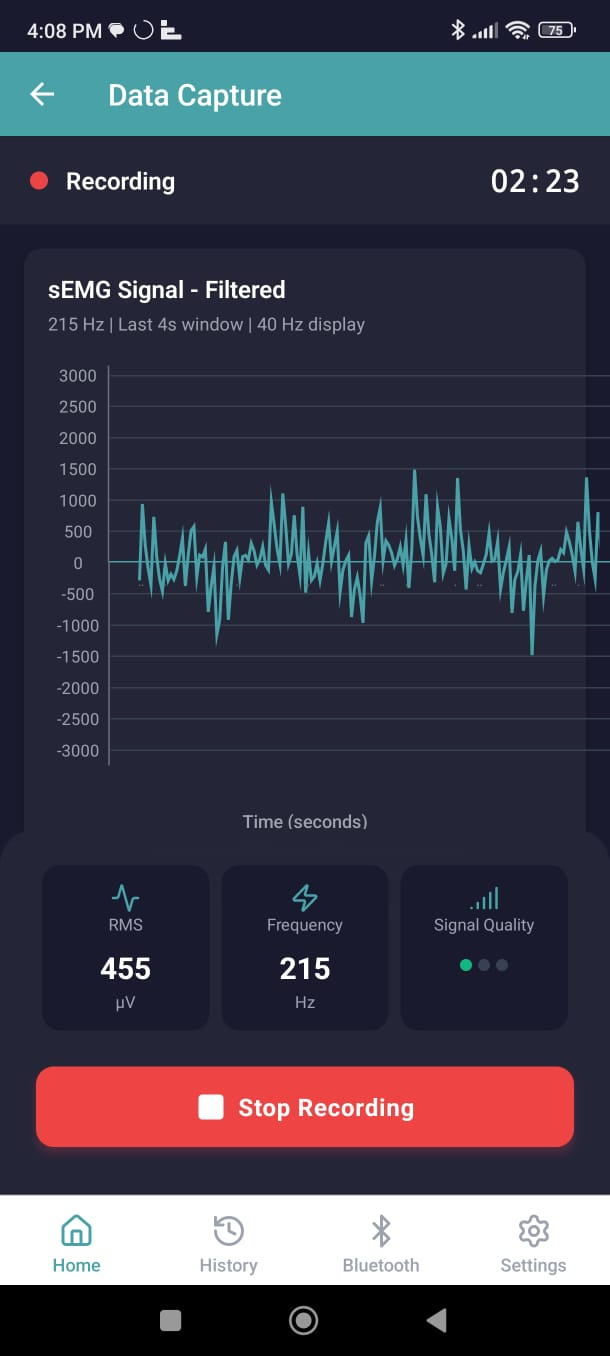
\includegraphics[scale=0.20]{figuras/telasIrisMobile/grafico_sem_contracao.jpeg}
}
\subfloat[Gráfico do sinal sEMG bíceps contraído]{
    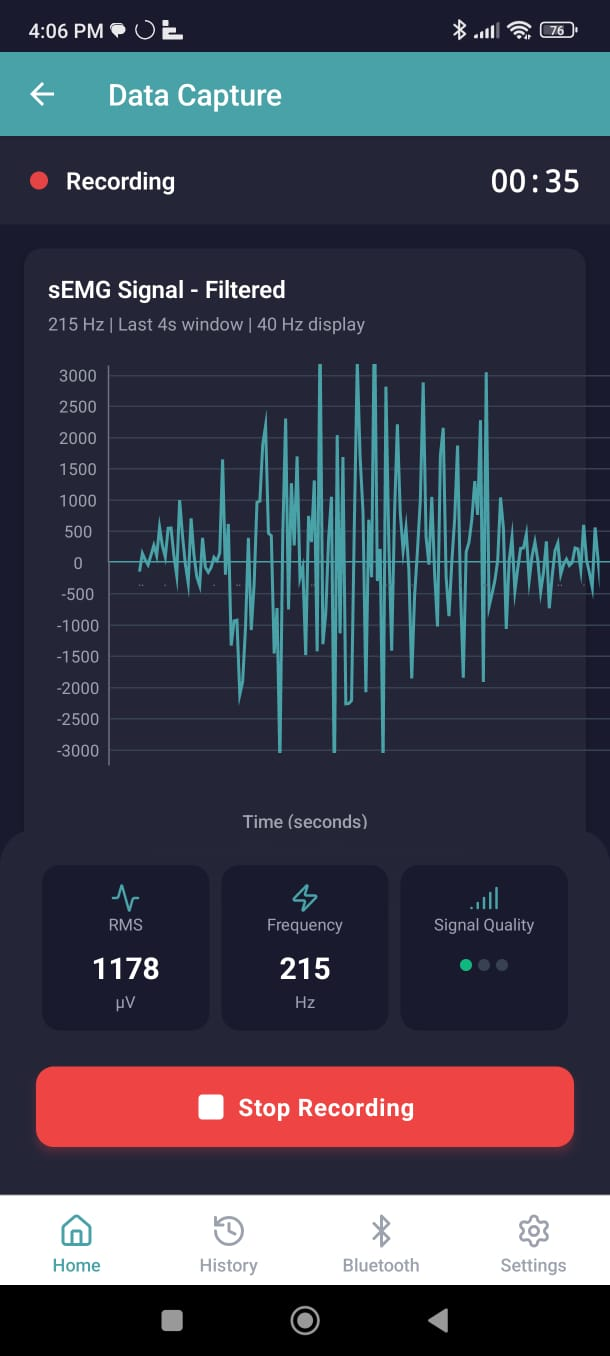
\includegraphics[scale=0.20]{figuras/telasIrisMobile/grafico_com_contracao.jpeg}
}\
\fonte{}
\end{figure}

A \texttt{HistoryScreen} (Figura~\ref{fig:irisMobileTelaHistorico}), apresentada sob o título \emph{Session History}, consolida visualmente o estado da sincronização discutido na Subseção~\ref{subsec:IRISMobileCaptura}. A tela é encabeçada por uma barra de busca que permite filtrar as sessões por voluntário ou data e organiza cada sessão como um cartão independente, contendo a data e hora de início, o nome do voluntário e a estrutura anatômica alvo; no canto superior direito do cartão é exibida a etiqueta colorida correspondente ao \texttt{sync\_status} da sessão (\textit{e.g.}, \emph{Synced}, em verde, com ícone de validação), e, em sessões em estado de falha, um botão \emph{Retry} alinhado à etiqueta permite reenfileirar a entidade ao próximo ciclo do \texttt{SyncService}. Cada cartão oferece, adicionalmente, uma ação de exportação local da sessão em arquivo \texttt{ZIP} (botão \emph{Export ZIP}), contendo os arquivos CSV das gravações e os metadados associados, recurso útil para análise \textit{offline} ou para o transporte do material adquirido a outras ferramentas externas ao NPI.

\begin{figure}[htpb]
\caption{Tela de histórico de coletas do IRIS \textit{Mobile}, com etiquetas indicativas do estado de sincronização de cada sessão.}
\label{fig:irisMobileTelaHistorico}
\centering
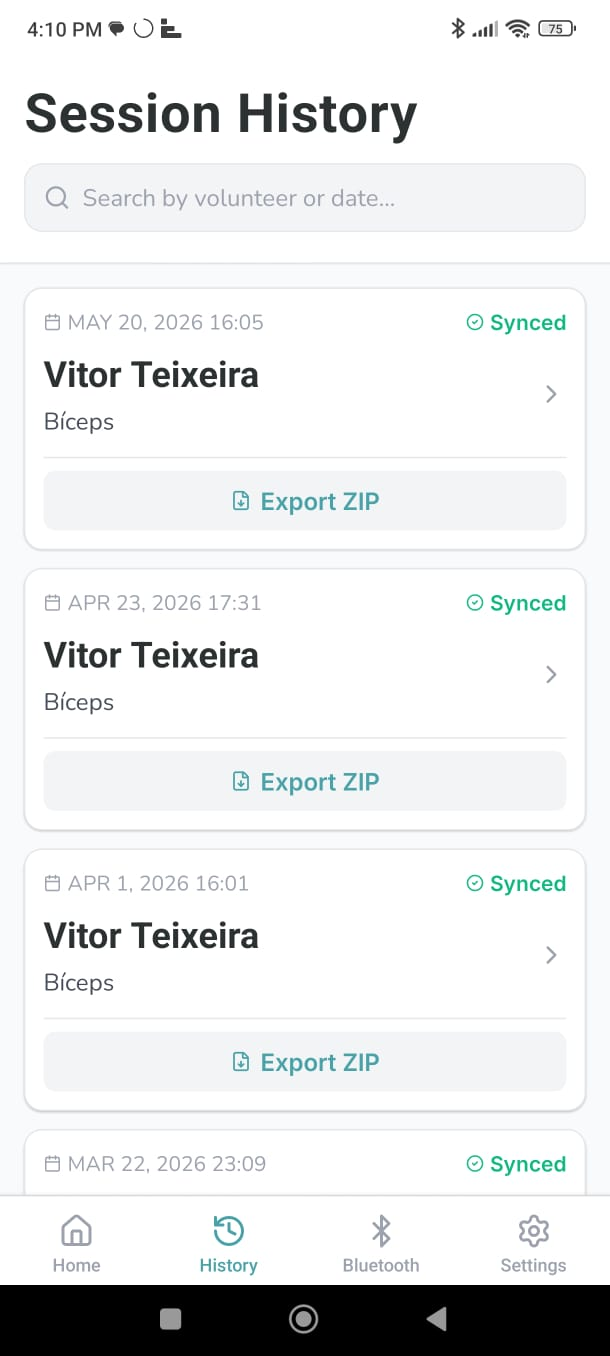
\includegraphics[scale=0.20]{figuras/telasIrisMobile/historico.jpeg}
\fonte{}
\end{figure}
